\section{Algorithm description}
\label{sec:desc}

The Fig. \ref{figurelabel_sys} shows a simplified block diagram of the proposed system. Two details are important, 
the use of the tracker window to initialize a segmentation procedure, and the use of this segmentation over the tracked window 
to perform a more precise motion flow computation in the interest pixels. The dotted line represents the possible interaction 
between precise flow information with the next tracker state. For instance, the current object flow can work as direction hint, and 
the segmentation information can be used to improve the sampling process of the learning stage in several trackers by detection methods \cite{c22}, and 
thus the tracker and motion flow algorithm can work for mutual enhancement.

\ifcsdef{r@accv_format}{

   \begin{figure}[thpb]
      \centering
      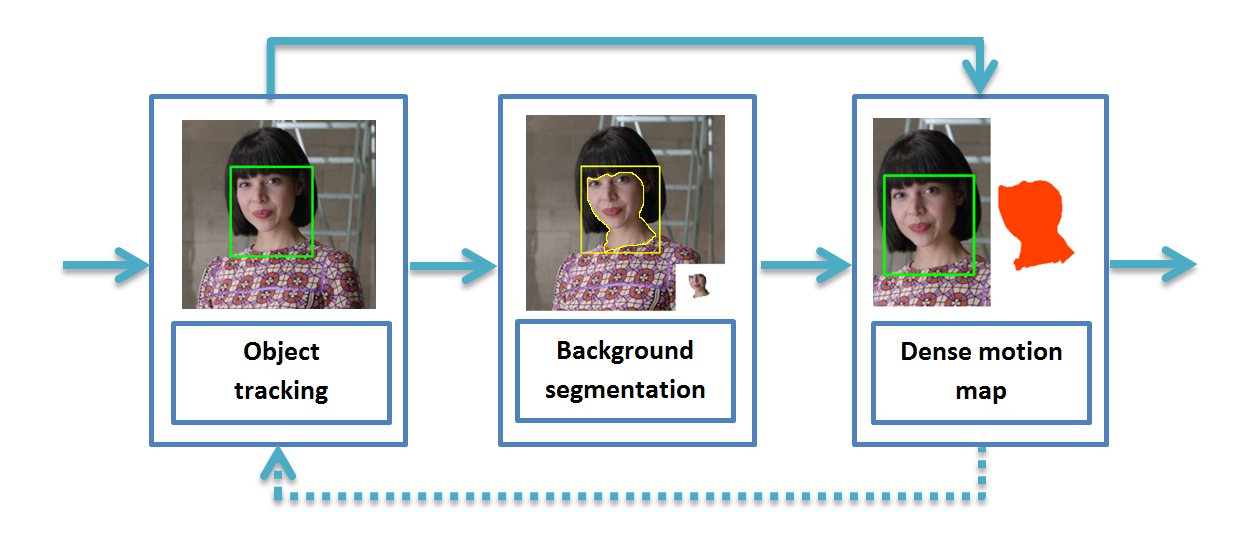
\includegraphics[width=1.00\textwidth]{../images/system.png}
      \caption{Block diagram of the proposed pipeline.}
      \label{figurelabel_sys}
   \end{figure}
}{
   \begin{figure}[thpb]
      \centering
      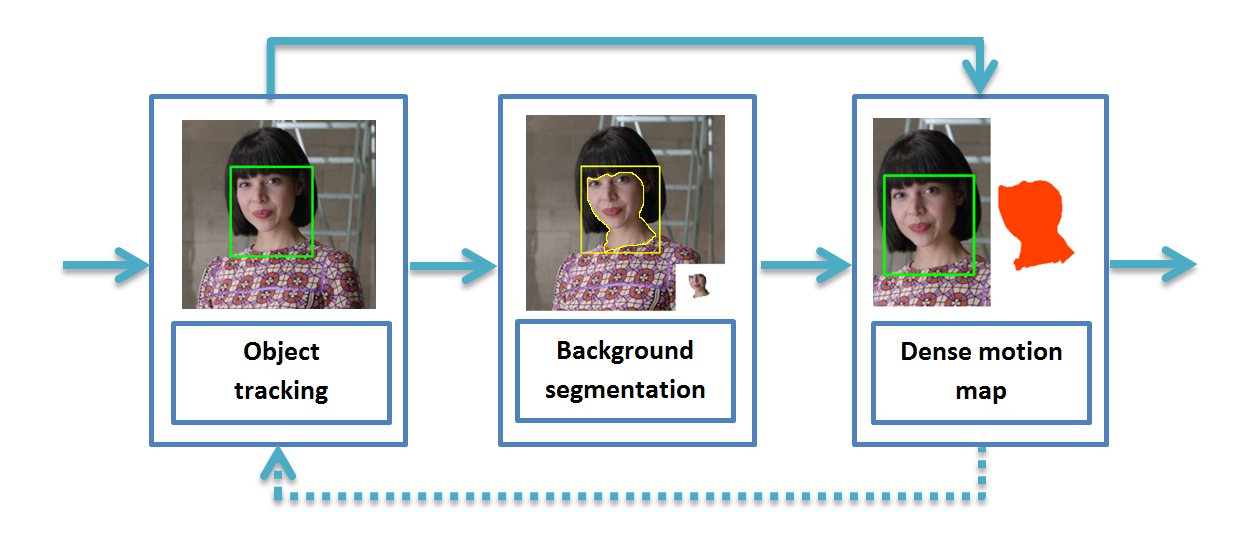
\includegraphics[width=0.5\textwidth]{../images/system.png}
      \caption{Block diagram of the proposed pipeline.}
      \label{figurelabel_sys}
   \end{figure}
}

The first step in the object flow pipeline can be selected according to specific need for a given application. We prefer, in general, tracking-by-detection methods 
like $Struck$ \cite{c22} or $MIL$ \cite{c23}, but other approaches could be followed. In the second place, for the object segmentation in video we propose the use 
of labelled background regions through the concept of superpixel flow, which is explained in the next section. Finally, the flow motion field is computed within the segmentation boundaries and long term dense 
point trajectories may be extracted from this.

